\begin{activity} \label{A:11.7.5} Consider the solid $S$ that is bounded by the parabolic cylinder $y = x^2$ and the planes $z=0$ and $z=1-y$ as shown in Figure \ref{F:11.7.TI_Example_2}. 
\begin{figure}[ht]
\begin{center}
%\resizebox{!}{2.0in}{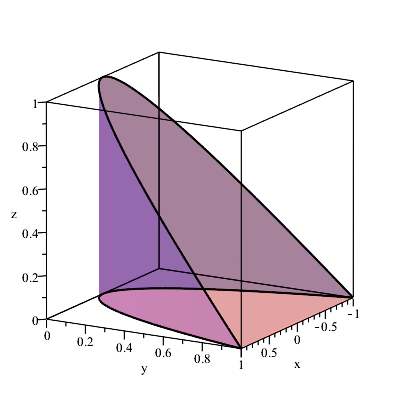
\includegraphics{11_7_TI_Example_2}}
  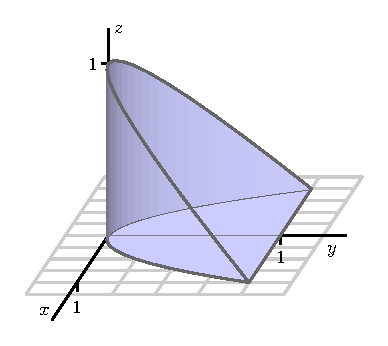
\includegraphics{figures/fig_11_7_solid.eps}
\end{center}
\caption{The solid bounded by $y = x^2$ and the planes $z=0$ and $z=1-y$.}
\label{F:11.7.TI_Example_2}
\end{figure}

Assume the density of $S$ is given by $\delta(x,y,z) = z$
    \ba
    \item Set up (but do not evaluate) an iterated integral that represents the mass of $S$.  Integrate first with respect to $z$, then $y$, then $x$  A picture of the projection of $S$ onto the $xy$-plane is shown in Figure \ref{F:11.7.TI_Example_2_xy}.

    \item Set up (but do not evaluate) an iterated integral that represents the mass of $S$.  In this case, integrate first with respect to $y$, then $z$, then $x$.  A picture of the projection of $S$ onto the $xz$-plane is shown in Figure \ref{F:11.7.TI_Example_2_xz}.


	\item Set up (but do not evaluate) an iterated integral that represents the mass of $S$.  A picture of the projection of $S$ onto the $yz$-plane is shown in Figure \ref{F:11.7.TI_Example_2_yz}.

	\item Which of these three orders of integration is the most natural to you?  Why?

	\ea

\begin{figure}[ht]
\begin{center}
\begin{minipage}{1.75in}
\begin{center}
%\resizebox{!}{1.7in}{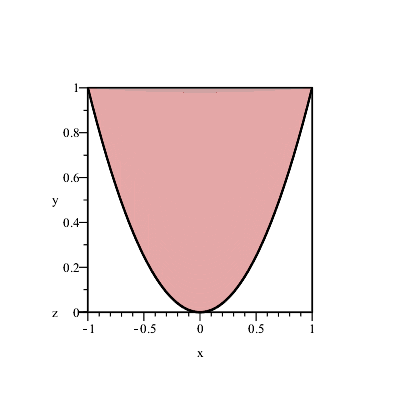
\includegraphics{11_7_TI_Example_2_xy}}
  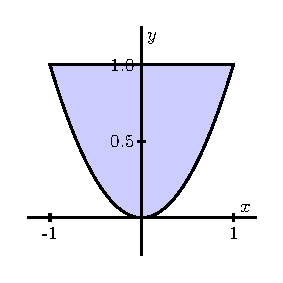
\includegraphics{figures/fig_11_7_solid_proj_1.eps}
\end{center}
\caption{Projecting $S$ onto the $xy$-plane.}
\label{F:11.7.TI_Example_2_xy}
\end{minipage} \hspace{0.1in}
\begin{minipage}{1.75in}
\begin{center}
%\resizebox{!}{1.7in}{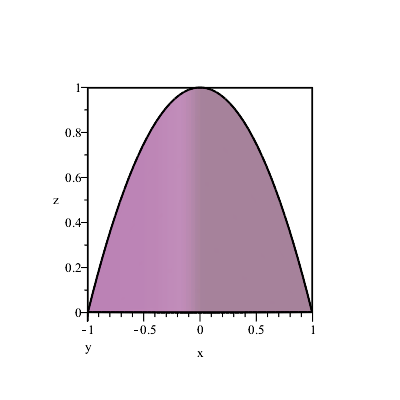
\includegraphics{11_7_TI_Example_2_xz}}
  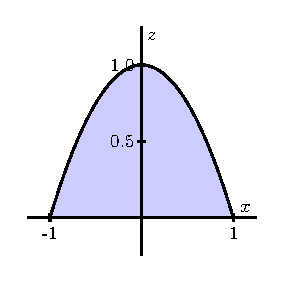
\includegraphics{figures/fig_11_7_solid_proj_2.eps}
\end{center}
\caption{Projecting $S$ onto the $xz$-plane.}
\label{F:11.7.TI_Example_2_xz}
\end{minipage} \hspace{0.1in}
\begin{minipage}{1.75in}
\begin{center}
%\resizebox{!}{1.7in}{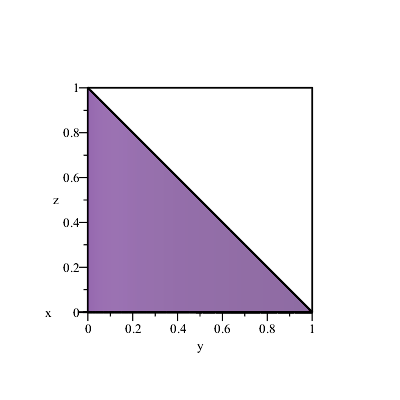
\includegraphics{11_7_TI_Example_2_yz}}
  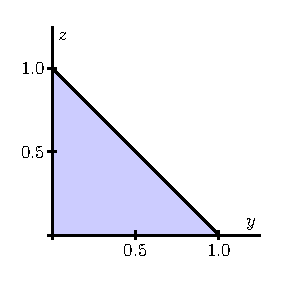
\includegraphics{figures/fig_11_7_solid_proj_3.eps}
\end{center}
\caption{Projecting $S$ onto the $yz$-plane.}
\label{F:11.7.TI_Example_2_yz}
\end{minipage}
\end{center}
\end{figure}


\end{activity}
\begin{smallhint}

\end{smallhint}
\begin{bighint}

\end{bighint}
\begin{activitySolution}
    \ba
    \item The iterated integral is 
\[\int_{-1}^{1} \int_{x^2}^{1} \int_{0}^{1-y} z \, dz \, dy \, dx.\]

    \item The iterated integral is 
\[\int_{0}^{1} \int_{0}^{1-x^2} \int_{x^2}^{1} z \, dy \, dz \, dx.\]

	\item The iterated integral is 
\[\int_{0}^{1} \int_{0}^{z} \int_{-\sqrt{y}}^{\sqrt{y}} z \, dx \, dy \, dz.\]

	\ea
\end{activitySolution}
\aftera
